\documentclass[12pt, titlepage, oneside]{article}
\usepackage[letterpaper, margin=1in]{geometry}
\usepackage{siunitx, booktabs, amsmath, enumitem, pdfpages, tabularx,caption, graphicx, pgfplots, textcomp}
\usepackage[siunitx]{circuitikz}
\sisetup{detect-weight=true, detect-family=true}
\usepackage{wrapfig}
\usepackage{mathrsfs}
\setlength\parindent{0pt}
\let\oldhat\hat
\let\oldvec\vec
\newcommand{\cross}{\bm{\times}}
\renewcommand{\hat}[1]{\oldhat{\mathbf{#1}}}
\usepackage{bm}
\renewcommand{\vec}[1]{\oldvec{\bm{#1}}}
\renewcommand{\hat}[1]{\oldhat{\bm{#1}}}
\renewcommand{\b}[1]{\textbf{#1}}

\begin{document}
\section*{25.1 Electric Potential and Potential Difference}
We know the force described by Coulombs law is conservative. Therefore, the force equation below is also conservative. A conservative force does the same work independent of path.
\begin{equation*}
\vec{F_E} = q \vec{E}
\end{equation*}
To get the potential energy on the system due to the $\vec{F_E}$, we use the definition of potential energy.
\begin{align*}
\Delta U = - \int_A^B \vec{F} \cdot d\vec{s}
\end{align*}
\noindent\fbox{%
	\parbox{\textwidth}{%
		\textbf{Change in Potential Energy}
\begin{align}
\Delta U = -q \int_A^B \vec{E} \cdot d \vec{s} = -q \vec{E} \cdot (\vec{B}-\vec{A})
\end{align}
$d \vec{s}$ is a very small displacement vector
}}
\\

\noindent  We only need to worry about the difference of potential at point A and point B due nature of conservative forces.
\\

\noindent For s given position of a charge in a field, there is potential energy, $U$ relative to the configuration of the system. Dividing by charge provides a physical quantity that depends only on the charges around that point. This is called the electric potential, or potential.\\

\noindent\fbox{%
	\parbox{\textwidth}{%
		\textbf{Electric Potential}
		\begin{align}
		V = \frac{U}{q} \hspace{1cm}\text{[1V = 1J/C]}
		\end{align}
}}
\\

\noindent The difference in electrical potential is the difference in potential energy as the charge $q$ does not change.`
\begin{align*}
\Delta V &= \frac{\Delta U}{q} = \dfrac{-q \int_A^B \vec{E} \cdot d \vec{s}}{q}
\end{align*}
Simplify the above to get,\\

\noindent\fbox{%
	\parbox{\textwidth}{%
		\textbf{Electrical Potential Difference}
		\begin{align}
		\Delta V &= \frac{\Delta U}{q} =-\int_A^B \vec{E} \cdot d \vec{s}
		\end{align}
}}
\newpage
So we know the external work being done is $W = \Delta U$
\begin{equation*}
W = q \Delta V
\end{equation*}
it would also be important to note the value of an electron volt.
\textbf{Electron volts are units of energy, not potential}
\begin{align*}
1\si{eV} = \SI{1.60e-19}{C\cdot V} = \SI{1.60e-19}{J}
\end{align*}
\section*{25.2 Potential Difference in a Uniform Electric Field}
Notice that when there is a uniform electric field and the charge moves in the direction of the field, 

\begin{wrapfigure}[0]{r}{0.5\textwidth}
	\begin{center}
		\vspace{-1.6cm}
		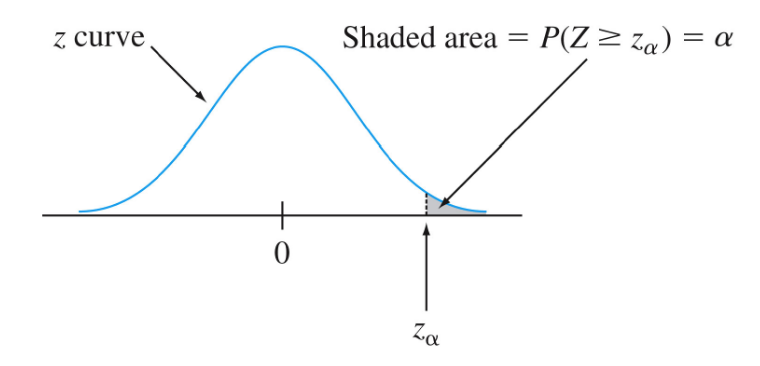
\includegraphics[scale=0.8]{1.png}
	\end{center}
\end{wrapfigure} 
\begin{align*}
\Delta V &= -\int_A^B \vec{E} \cdot d\vec{s} \\
		 &= -\int_A^B E ds (\cos 0^{\circ}) \\
		 &= -\int_A^B Eds \\
		 &= -E \int_A^B ds\hspace{7cm}
\end{align*} 
\\

\noindent\fbox{%
	\parbox{\textwidth}{%
		\textbf{Uniform Electric Field, Electric Potential Difference}
		\begin{align}
		\Delta V = -Ed
		\end{align}
		Where d is the distance the charge travelled in the direction of the field.
	}}
\\
\\
\
\noindent The above equation makes sense from a theoretical standpoint because field lines always point from high electric potential to low electric potential, $V_B < V_A$. From this we can also see that,
\begin{align*}
\Delta U = q \Delta V = q (-Ed) = -qEd
\end{align*}
As the charge modes towards lower potential, the potential decreases. This makes sense because if we released a proton from rest in this system, it will accelerate and gain kinetic energy, therefore potential needs to drop to obey conservation of energy.\\

\newpage

\begin{wrapfigure}[14]{r}{0.4\textwidth}
	\begin{center}
	\vspace{-1cm}
		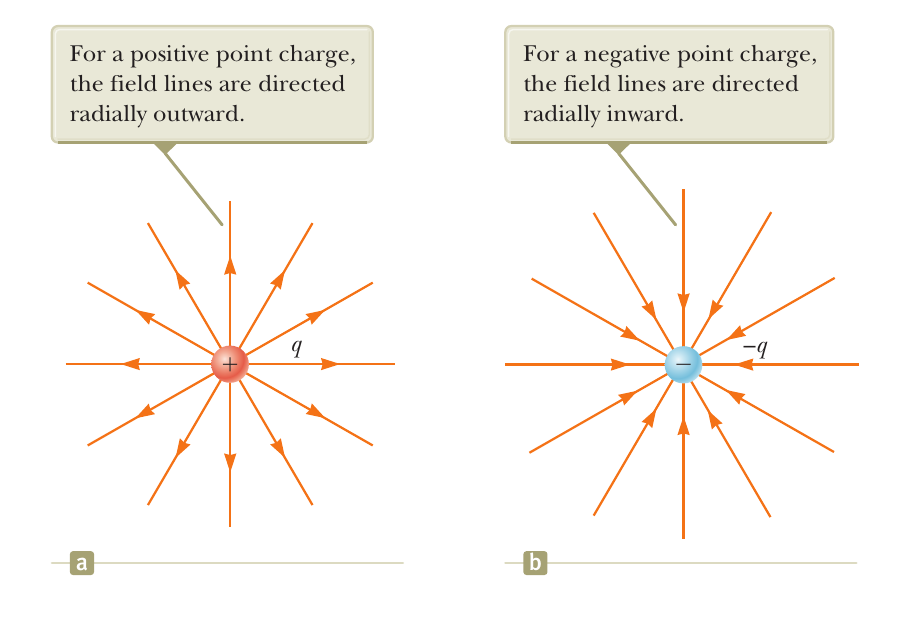
\includegraphics[scale=1]{2.png}
	\end{center}
\end{wrapfigure} 
\noindent If the charge had initial speed in a direction not parallel to field lines, we need to use the equation,
\begin{equation*}
\Delta V = - \int_A^B \vec{E} \cdot d\vec{s} = -\vec{E} \cdot \vec{s}
\end{equation*}
The vector $\vec{s}$ is simply the path of travel
\begin{equation*}
\Delta U = q \Delta V = -q \vec{E} \cdot \vec{s}
\end{equation*}
Additional notes in this chapter include the fact that equipotential lines have $\Delta V = 0$ as everywhere along the line $V$ is the same. Lastly, equipotential lines are usually perpendicular to uniform fields as $\cos 90^{\circ} = 0$.
\section*{25.3 Electric Potential and Potential Energy Due to Point Charges}

\begin{wrapfigure}[20]{r}{0.4\textwidth}
	\begin{center}
		\vspace{-2cm}
		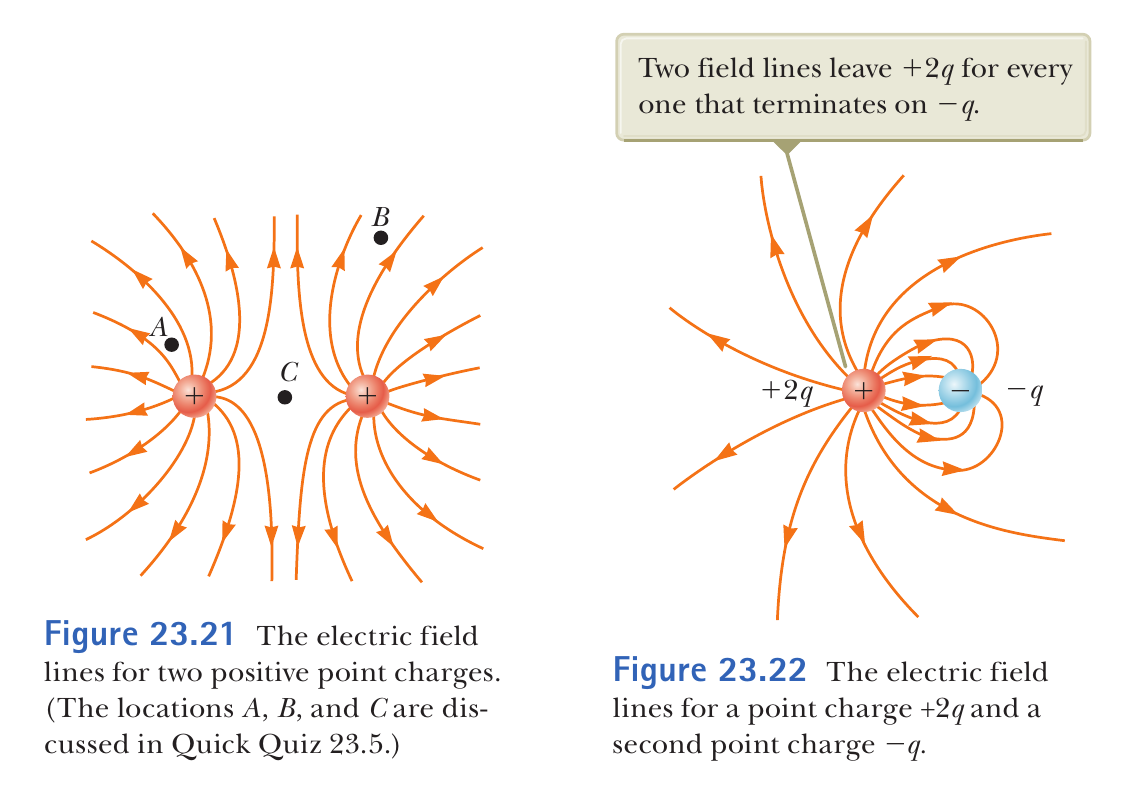
\includegraphics[scale=1]{3.png}
	\end{center}
\end{wrapfigure} 
To find electric potential at a distance $r$, we can recall from previous chapters,
\begin{align*}
V_B - V_A = - \int_A^B \vec{E} \cdot d\vec{s}
\end{align*}
So, we can also rewrite this as,
\begin{align*}
\vec{E} \cdot d \vec{s} = k_e \dfrac{q}{r^2}\hat{r} \cdot d \vec{s}
\end{align*}
Since the magnitude of $\hat{r}$ is 1, we can therefore write $\hat{r} d \vec{s} = ds \cos\theta$. From the figure on the right, we can see that $\theta$ is just the angle between the radius from the charge and the path it takes to change electric potential. (conservative field)
\begin{align*}
V_B - V_A &= - k_e q \int_A^B \dfrac{dr}{r^2} = k_e \frac{q}{r} \Big|_A^B\\
V_B - V_A &= k_e q \Bigg[\frac{1}{r_B}-\frac{1}{r_A}\Bigg]
\end{align*}
If we choose a point A very far off such that $ r=\infty$ then $V_A = 0$, therefore,
\newpage
\noindent\fbox{%
	\parbox{\textwidth}{%
			\textbf{Electric Potential}
			\begin{equation}
			V = k_e \frac{q}{r}
			\end{equation}
	}}.
\\

\noindent If there is more than one charge, we can simply sum all the charges to find the total electric potential at a point.

\begin{align*}
V = k_e \sum_i \frac {q_i}{r_i}
\end{align*}
Therefore, using this as the basis, we can get the \textbf{electrical potential energy}
\begin{align*}
U_f - U_i = W = Q\Delta V \rightarrow U - 0 = Q\Bigg(k_e\frac{q}{r}\Bigg)
\end{align*}
\noindent\fbox{%
	\parbox{\textwidth}{%
		\textbf{Electric Potential ENERGY}
		\begin{align}
	U = K_e \frac{Qq}{r}
\end{align}
}}	\\

\begin{wrapfigure}[12]{r}{0.4\textwidth}
	\begin{center}\vspace{-1.1cm}
		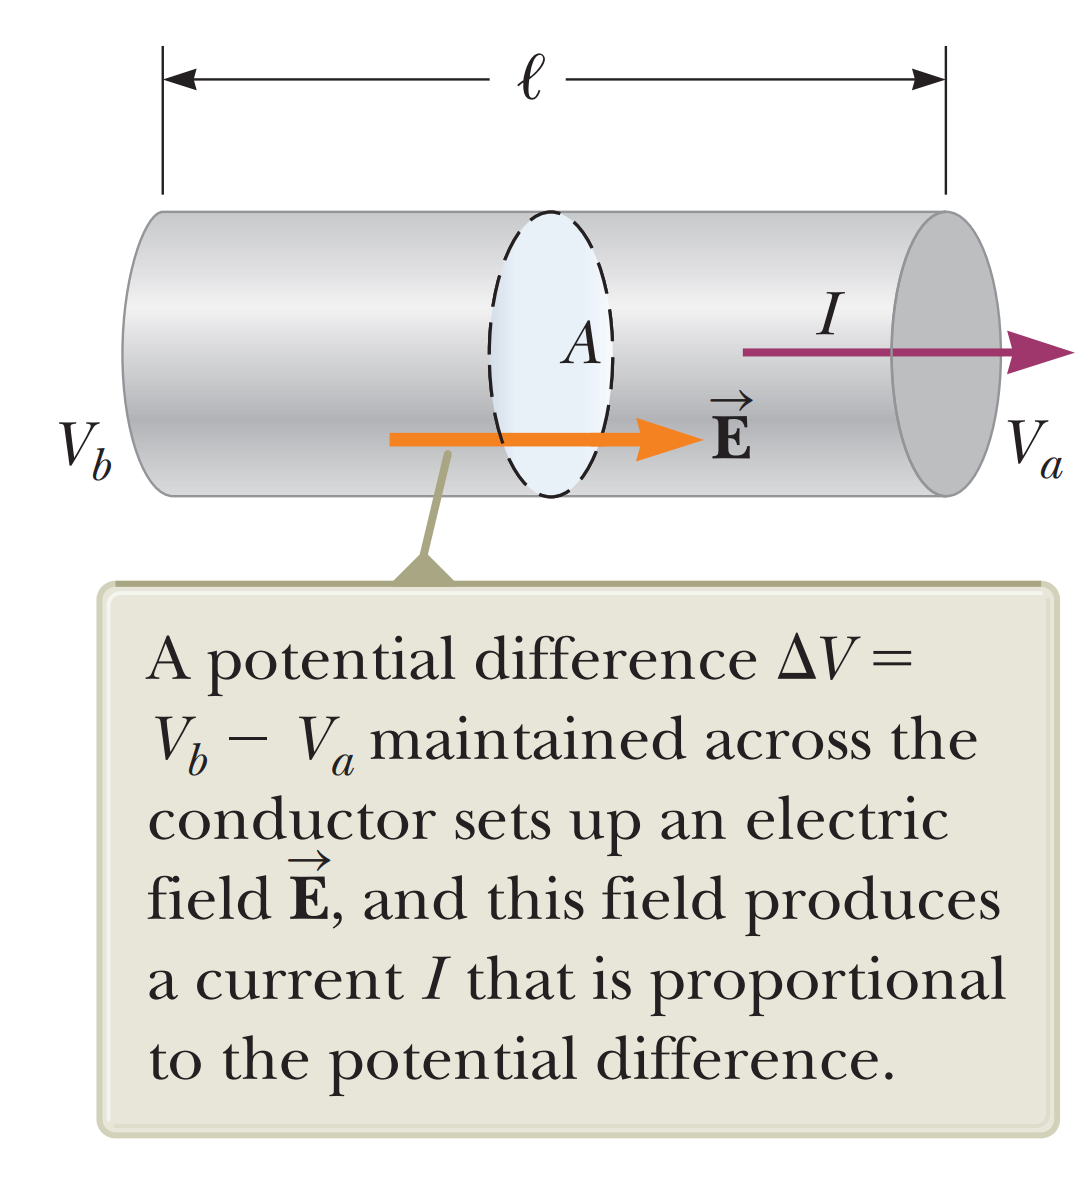
\includegraphics[scale=0.3]{4.png}
	\end{center}
\end{wrapfigure} 
If there is multiple charges, and you want to find the total electric potential energy of the system, we can simply sum all the electric potential energies
\begin{align*}
U = k_e \Bigg(\frac{q1q2}{r_{12}} + \frac{q1q3}{r_{13}} + \frac{q2q3}{r_{23}} \Bigg)
\end{align*}

This answer can be interpreted by imagining that initially, q1 is at the same position as shown on the figure, but q2 and q3 are at infinity. What is the energy required to push those to charge into place.
\section*{25.4 Obtaining the Value of the Electric Field from the Electric Potential}
Given a very small displacement d$\vec{s}$ the potential does not change much, therefore it changes a d$V$. For a more simple derivation, we can say that $E$ is a field which only exists in the x direction, therefore d$\vec{s}$ becomes dx.
\newpage
\noindent
Using old equations in the previous chapeters, we have seen that,
\begin{align*}
dV = -\vec{E} \cdot d\vec{s}
\end{align*}
With our assumptions, we can rewrite this as,
\begin{align*}
E_x = -\frac{dv}{dx}
\end{align*}
If there is more than one component, we can simply take the partial derivatives with respect to each component.
\\

\noindent\fbox{%
	\parbox{\textwidth}{%
	\textbf{Obtaining the Electric Field}
	\begin{align}
	E_x = -\frac{\partial V}{\partial x} \hspace{1cm}
	E_y = -\frac{\partial V}{\partial y}
	\hspace{1cm}
	E_z = -\frac{\partial V}{\partial x}\\[5pt]
	\vec{E} = -\nabla V = -\Bigg(\hat{i}\frac{\partial}{\partial x} + \hat{j}\frac{\partial}{\partial y} +
	\hat{k}\frac{\partial}{\partial z}\Bigg)V 
	\hspace{15pt}
	\end{align}	
}}
\\

\noindent
From this chapter, we also see that all equipotential lines are perpendicular to field lines.
\begin{center}
	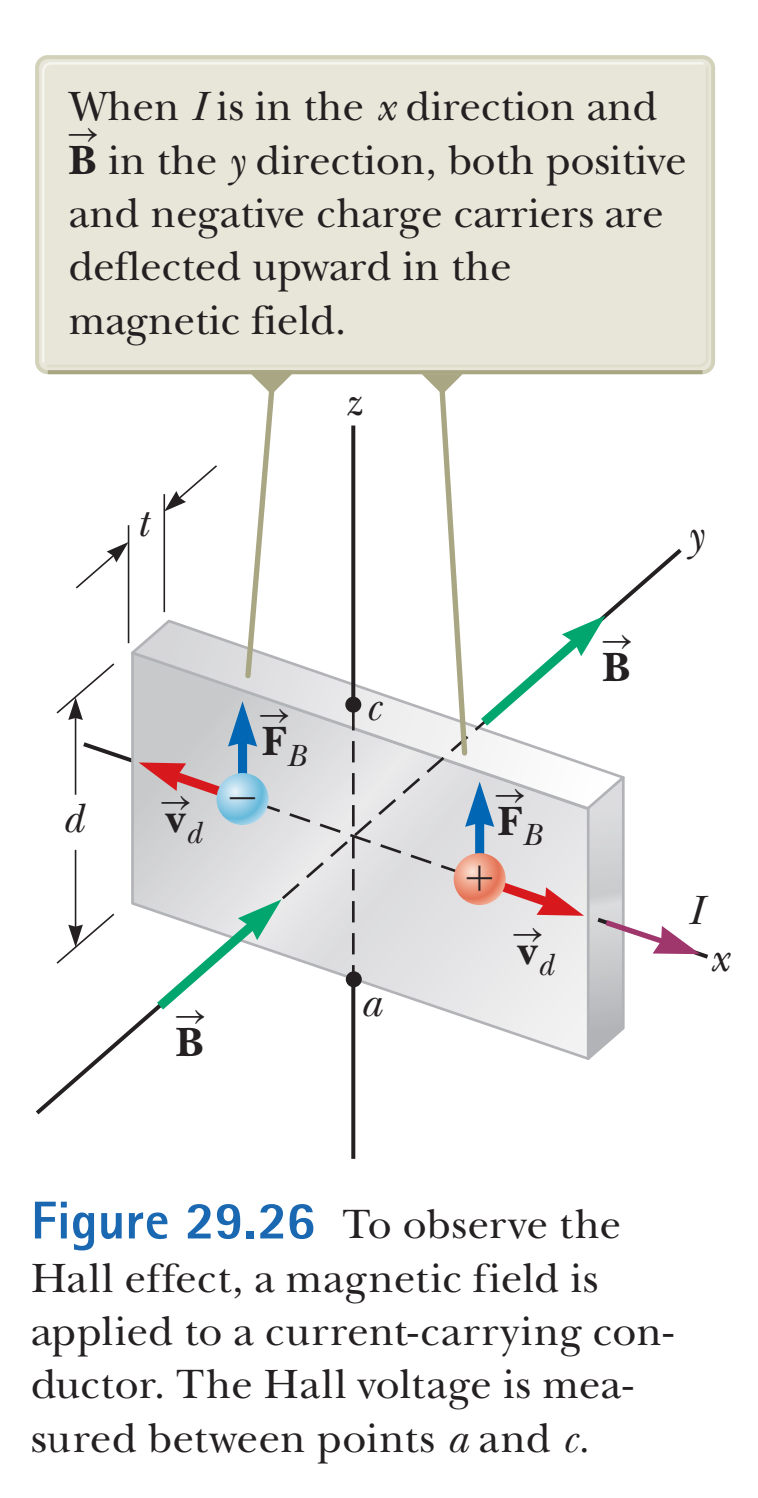
\includegraphics[scale=.55]{5.png}
\end{center}

\end{document}